\documentclass{article}

%-------------------------%
% PREAMBUŁA --------------%
%-------------------------%
\usepackage[utf8]{inputenc}
\usepackage[OT4]{polski}
\usepackage{caption}
\usepackage{amsmath}
\usepackage{tikz}
\usepackage{subcaption}
\usepackage{tabularx}
\usepackage{caption}
\usepackage{array}
\usepackage{hyperref}
\usepackage{graphicx}
\usepackage{fancyhdr}
\usepackage[justification=centering]{caption}
\usepackage[margin=60pt]{geometry}
\usepackage{longtable}



%\usepackage[T1]{fontenc}
%\usepackage{amsthm}
%\theoremstyle{plain}
%\usepackage{enumitem}
%\captionsetup[table]{skip=-4pt}
%\usepackage{tabulary}
%\usepackage{sidecap}
%\usepackage{gensymb}
%\usepackage{wrapfig}
%\usepackage{lastpage}
%\usepackage{gensymb}
%\usepackage{lipsum}
%\pagestyle{fancy}


\newlength{\RoundedBoxWidth}
\newsavebox{\GrayRoundedBox}
\newenvironment{GrayBox}[1][\dimexpr\textwidth-4.5ex]%
   {\setlength{\RoundedBoxWidth}{\dimexpr#1}
    \begin{lrbox}{\GrayRoundedBox}
       \begin{minipage}{\RoundedBoxWidth}}%
   {   \end{minipage}
    \end{lrbox}
    \begin{center}
    
\begin{tikzpicture}%
       \draw node[draw=black,fill=black!1,rounded corners,%
             inner sep=2ex,text width=\RoundedBoxWidth]%
             {\usebox{\GrayRoundedBox}};
    \end{tikzpicture}
    \end{center}}

%------- Typy kolumn do ustawiania szerokości ------- %
\newcolumntype{L}[1]{>{\raggedright\let\newline\\\arraybackslash\hspace{0pt}}m{#1}}
\newcolumntype{C}[1]{>{\centering\let\newline\\\arraybackslash\hspace{0pt}}m{#1}}
\newcolumntype{R}[1]{>{\raggedleft\let\newline\\\arraybackslash\hspace{0pt}}m{#1}}








\begin{document}

%-------------------------%
%Tabela nagłówkowa -------%
%-------------------------%

\begin{table}[h]
\begin{tabular}{|l|l|l|l|l|l|}
\hline
\begin{tabular}[c]{@{}l@{}}
Wydział:\\ WFiIS\end{tabular} &
\multicolumn{2}{l|}{\begin{tabular}[c]{@{}l@{}}
Imię i nazwisko:\\ 1. Axel Zuziak\\ 2. Marcin Węglarz \end{tabular}} 
& Rok \textbf{II}         
& Grupa \textbf{B}          
& Zespół \textbf{03}      \\ \hline
\textbf{\begin{tabular}[c]{@{}l@{}}
LABOLATORIUM\\ TECHNIK \\ JĄDROWYCH\end{tabular}} &
\multicolumn{4}{l|}{ Temat:\textbf{ Wyznaczanie czasu połowicznego rozpadu
		izotopów krótkotrwałych.} }                                                                                                                       & \multicolumn{1}{c|}{\begin{tabular}[c]{@{}c@{}}
Nr ćwiczenia\\ \textbf{1+9}
\end{tabular}} \\ \hline
\begin{tabular}[c]{@{}c@{}}
Data wykonania:\\ 04.03.2015
\end{tabular} &
\begin{tabular}[c]{@{}c@{}}
 Data oddania:\\ 18.03.2015
\end{tabular} &
\begin{tabular}[c]{@{}c@{}}
Zwrot do poprawy: \\ 
\end{tabular}                                 
& 
\begin{tabular}[c]{@{}c@{}}
Data oddania: \\ 
\end{tabular}&
\begin{tabular}[c]{@{}c@{}}
Data zaliczenia:\\
\end{tabular}& 
\begin{tabular}[c]{@{}c@{}}
OCENA:\\
\end{tabular}       
\\ & & & & & \\ \hline
\end{tabular}
\end{table}
%-----Koniec tabeli------

\section{Statystyczny charakter rozpadów promieniotwórczych}
\subsection{Cel ćwiczenia}
Celem ćwiczenia jest praktyczne zapoznanie się ze statystycznym charakterem rozpadów promieniotwórczych oraz wyznaczaniem histogramów rozkładów Poissona i Gaussa. Wyznaczono również charakterystykę licznika Geigera-Mullera.
\subsection{Wstęp teoretyczny}
Charakterystyką licznika Geigera-Mullera nazywamy zależność między częstością zliczeń rejestrowanych impulsów i napięciem zasilania licznika, przy stałym strumieniu padających na licznik cząstek i stałym poziomie progu dyskryminacji elektronicznej. Wykres [\ref{charakterystyka}] przedstawia prostoliniowy odcinek o niewielkim nachyleniu zwany $plateau$ licznika. Wartość $U_A$ nazywamy progiem geigerowskim. Nachylenie plateau $\alpha$ jest zdefiniowane jako przyrost liczby zliczeń przypadający na 100V wzrostu napięcia zasilania w zakresie plateau:
\begin{equation}
\label{nachylenie}
	 \alpha = \frac{(J_B - J_A)}{J_A}
\end{equation}
Rozkład Poissona jest to dyskretny rozkład prawdopodobieństwa, wyrażający prawdopodobieństwo szeregu zdarzeń, gdy występują one ze znaną średnią częstością. Wzór opisujący taki rozkład można zapisać:
\begin{equation}
\label{poisson}
	f(k,\lambda) = \frac{\lambda^k \cdot e^{-k}}{k!}
\end{equation}
Rozkład Gaussa jest w przeciwieństwie do rozkładu Poissona rozkładem ciągłym. Jego maksimum przypada na wartość oczekiwaną:
\begin{equation}
	\label{gauss}
	\Phi_{\mu,\sigma}(x) = \frac{1}{\sigma\sqrt{2\pi}}\exp{\left[\frac{-(x-\mu)^2}{2\sigma^2} \right]}
\end{equation}
Często stosowanym testem statystycznym jest test chi-kwadrat ($\chi^2$). Pozwala on określić czy wyniki danych pomiarów są zgodne, na określonym przedziale ufności z wynikami oczekiwanymi.
\begin{equation}
	\label{chi}
	\chi^2 = \sum_{i=1}^{r}\frac{(x_i - x_{oi})^2}{x_{oi}}
\end{equation}
Gdzie $x_i$ to wartości pomiarowe danej wielkości, $x_{oi}$ wartość oczekiwana tej wielkości podlegającej określonemu rozkładowi statystycznemu, natomiast $r$ to liczba pomiarów. Korzystając z tabel statystycznych możemy określić wartość $\chi^2_\alpha$. Jeżeli $\chi^2 < \chi^2_\alpha$ to nie mamy podstaw do odrzucenia założonej hipotezy. Można zatem przyjąć, że nie występują tu żadne inne rodzaje błędów oprócz błędów o charakterze fluktuacji statystycznych.
\begin{figure}[h!]
	\centering
	\label{charakterystyka}
	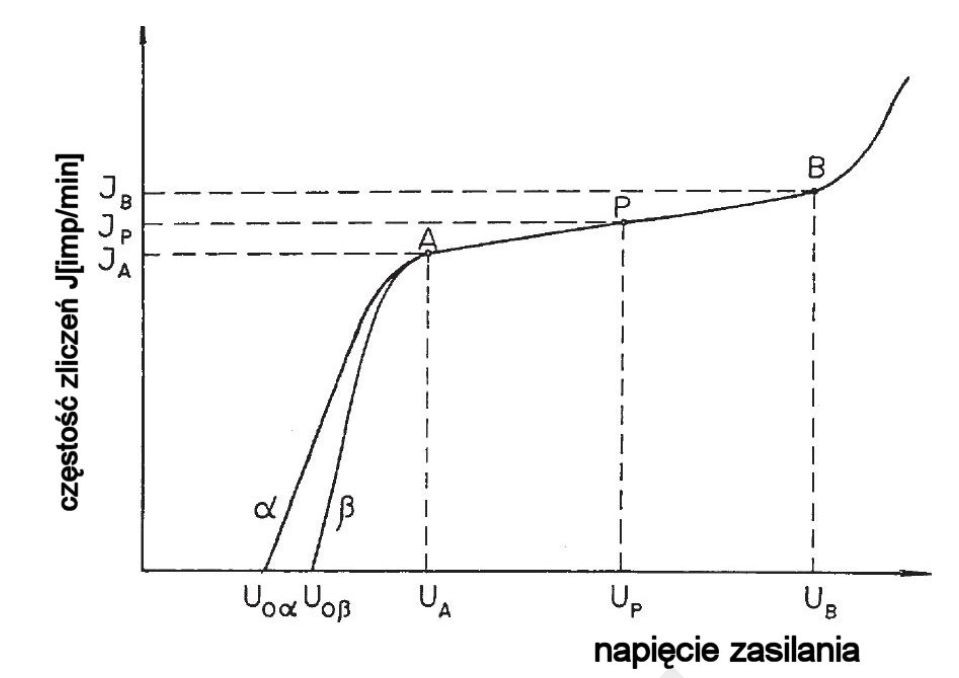
\includegraphics[width = 0.5\linewidth]{images/charakterystyka}
	\caption{Charakterystyka licznika Geigera-Mullera [\ref{uklad}]}
\end{figure}
\subsection{Wykonanie ćwiczenia}
Ćwiczenie rozpoczęto od zapoznania się z układem pomiarowym składającym się z:
\begin{itemize}
	\item \textbf{Domek pomiarowy}
	\item \textbf{Licznik Geigera-Mullera}
	\item \textbf{Wtórnik}
	\item \textbf{Zasilacz wysokiego napięcia}
	\item \textbf{Dyskryminator amplitudy}
	\item \textbf{Przelicznik}
	\item \textbf{Zasilacz niskiego napięcia}
\end{itemize}
\begin{figure}[h!]
	\centering
	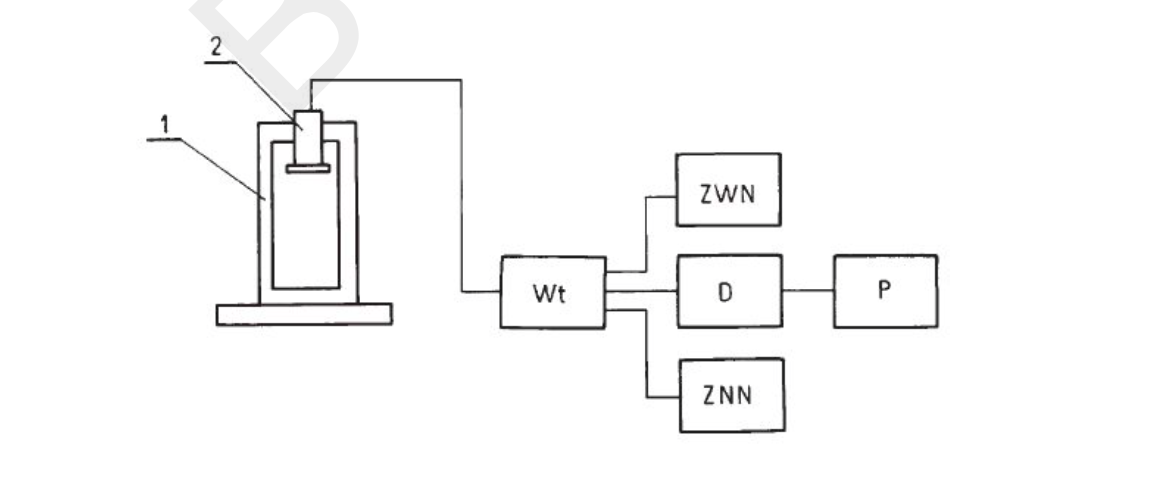
\includegraphics[width = 0.7\linewidth]{images/uklad}
	\caption{Schemat blokowy zestawu pomiarowego [\ref{uklad}]}
\end{figure}
Umieszczono źródło punktowe $^{137}$Cs w domku pomiarowym blisko licznika. W celu określenia napięcia progowego ustawiono długi czas pomiaru wynoszący 1000s i powoli zwiększano napięcie. Następnie wyznaczono charakterystykę licznika przeprowadzając pomiary co 20V w zakresie od 60V poniżej napięcia progowego do 200V powyżej tego napięcia. Czas trwania pojedynczego pomiaru wyznaczono tak, aby liczba zliczeń w plateau wynosiła około 1000. Następnie źródło umieszczono na zewnątrz domku pomiarowego w celu osiągnięcia średnio jednego zliczenia na sekundę. Wykonano 100 takich jednosekundowych pomiarów. Kolejno wykonano 100 pomiarów przy źródle umieszczonym w domku na samym dole oraz 200 pomiarów przy źródle umieszczonym na samej górze.
\newpage
\subsection{Wyniki pomiarów}
\begin{itemize}
	\item \textbf{Wyznaczenie charakterystyki licznika G-M}
\begin{table}[h!]
\centering
	\label{plateau}
	\caption{Wyniki pomiarów zliczeń w zależności od napięcia.}
	\begin{tabular}{|C{2cm}|C{2cm}|C{2.5cm}|C{3cm}|}\hline
				&	Napięcie [V] & Liczba zliczeń & Liczba zliczeń na sekundę \\ \hline
		1	&	1200	&	0		&	0,0 \\ \hline
		2	&	1220	&	0		&	0,0 \\ \hline
		3	&	1240	&	0		&	0,0 \\ \hline
		4	&	1260	&	56		&	2,8 \\ \hline
		5	&	1280	&	808		&	40,4 \\ \hline
		6	&	1300	&	857		&	42,9 \\ \hline
		7	&	1320	&	900		&	45,0 \\ \hline
		8	&	1340	&	857		&	42,9 \\ \hline
		9	&	1360	&	891		&	44,6 \\ \hline
		10	&	1380	&	866		&	43,3 \\ \hline
		11	&	1400	&	907		&	45,4 \\ \hline
		12	&	1420	&	920		&	46,0 \\ \hline
		13	&	1440	&	927		&	46,4 \\ \hline
		14	&	1460	&	907		&	45,4 \\ \hline
	\end{tabular}
\end{table}

\begin{figure}[h!]
	\fontsize{6}{8}\selectfont % zmniejszam czcionke
	\centering
	\resizebox{0.7\textwidth}{!}{% GNUPLOT: LaTeX picture with Postscript
\begingroup
  \makeatletter
  \providecommand\color[2][]{%
    \GenericError{(gnuplot) \space\space\space\@spaces}{%
      Package color not loaded in conjunction with
      terminal option `colourtext'%
    }{See the gnuplot documentation for explanation.%
    }{Either use 'blacktext' in gnuplot or load the package
      color.sty in LaTeX.}%
    \renewcommand\color[2][]{}%
  }%
  \providecommand\includegraphics[2][]{%
    \GenericError{(gnuplot) \space\space\space\@spaces}{%
      Package graphicx or graphics not loaded%
    }{See the gnuplot documentation for explanation.%
    }{The gnuplot epslatex terminal needs graphicx.sty or graphics.sty.}%
    \renewcommand\includegraphics[2][]{}%
  }%
  \providecommand\rotatebox[2]{#2}%
  \@ifundefined{ifGPcolor}{%
    \newif\ifGPcolor
    \GPcolortrue
  }{}%
  \@ifundefined{ifGPblacktext}{%
    \newif\ifGPblacktext
    \GPblacktextfalse
  }{}%
  % define a \g@addto@macro without @ in the name:
  \let\gplgaddtomacro\g@addto@macro
  % define empty templates for all commands taking text:
  \gdef\gplbacktext{}%
  \gdef\gplfronttext{}%
  \makeatother
  \ifGPblacktext
    % no textcolor at all
    \def\colorrgb#1{}%
    \def\colorgray#1{}%
  \else
    % gray or color?
    \ifGPcolor
      \def\colorrgb#1{\color[rgb]{#1}}%
      \def\colorgray#1{\color[gray]{#1}}%
      \expandafter\def\csname LTw\endcsname{\color{white}}%
      \expandafter\def\csname LTb\endcsname{\color{black}}%
      \expandafter\def\csname LTa\endcsname{\color{black}}%
      \expandafter\def\csname LT0\endcsname{\color[rgb]{1,0,0}}%
      \expandafter\def\csname LT1\endcsname{\color[rgb]{0,1,0}}%
      \expandafter\def\csname LT2\endcsname{\color[rgb]{0,0,1}}%
      \expandafter\def\csname LT3\endcsname{\color[rgb]{1,0,1}}%
      \expandafter\def\csname LT4\endcsname{\color[rgb]{0,1,1}}%
      \expandafter\def\csname LT5\endcsname{\color[rgb]{1,1,0}}%
      \expandafter\def\csname LT6\endcsname{\color[rgb]{0,0,0}}%
      \expandafter\def\csname LT7\endcsname{\color[rgb]{1,0.3,0}}%
      \expandafter\def\csname LT8\endcsname{\color[rgb]{0.5,0.5,0.5}}%
    \else
      % gray
      \def\colorrgb#1{\color{black}}%
      \def\colorgray#1{\color[gray]{#1}}%
      \expandafter\def\csname LTw\endcsname{\color{white}}%
      \expandafter\def\csname LTb\endcsname{\color{black}}%
      \expandafter\def\csname LTa\endcsname{\color{black}}%
      \expandafter\def\csname LT0\endcsname{\color{black}}%
      \expandafter\def\csname LT1\endcsname{\color{black}}%
      \expandafter\def\csname LT2\endcsname{\color{black}}%
      \expandafter\def\csname LT3\endcsname{\color{black}}%
      \expandafter\def\csname LT4\endcsname{\color{black}}%
      \expandafter\def\csname LT5\endcsname{\color{black}}%
      \expandafter\def\csname LT6\endcsname{\color{black}}%
      \expandafter\def\csname LT7\endcsname{\color{black}}%
      \expandafter\def\csname LT8\endcsname{\color{black}}%
    \fi
  \fi
  \setlength{\unitlength}{0.0500bp}%
  \begin{picture}(7370.00,5102.00)%
    \gplgaddtomacro\gplbacktext{%
      \csname LTb\endcsname%
      \put(946,704){\makebox(0,0)[r]{\strut{}$0$}}%
      \csname LTb\endcsname%
      \put(946,1117){\makebox(0,0)[r]{\strut{}$100$}}%
      \csname LTb\endcsname%
      \put(946,1531){\makebox(0,0)[r]{\strut{}$200$}}%
      \csname LTb\endcsname%
      \put(946,1944){\makebox(0,0)[r]{\strut{}$300$}}%
      \csname LTb\endcsname%
      \put(946,2357){\makebox(0,0)[r]{\strut{}$400$}}%
      \csname LTb\endcsname%
      \put(946,2771){\makebox(0,0)[r]{\strut{}$500$}}%
      \csname LTb\endcsname%
      \put(946,3184){\makebox(0,0)[r]{\strut{}$600$}}%
      \csname LTb\endcsname%
      \put(946,3597){\makebox(0,0)[r]{\strut{}$700$}}%
      \csname LTb\endcsname%
      \put(946,4010){\makebox(0,0)[r]{\strut{}$800$}}%
      \csname LTb\endcsname%
      \put(946,4424){\makebox(0,0)[r]{\strut{}$900$}}%
      \csname LTb\endcsname%
      \put(946,4837){\makebox(0,0)[r]{\strut{}$1000$}}%
      \csname LTb\endcsname%
      \put(1078,484){\makebox(0,0){\strut{}$1200$}}%
      \csname LTb\endcsname%
      \put(2061,484){\makebox(0,0){\strut{}$1250$}}%
      \csname LTb\endcsname%
      \put(3043,484){\makebox(0,0){\strut{}$1300$}}%
      \csname LTb\endcsname%
      \put(4026,484){\makebox(0,0){\strut{}$1350$}}%
      \csname LTb\endcsname%
      \put(5008,484){\makebox(0,0){\strut{}$1400$}}%
      \csname LTb\endcsname%
      \put(5991,484){\makebox(0,0){\strut{}$1450$}}%
      \csname LTb\endcsname%
      \put(6973,484){\makebox(0,0){\strut{}$1500$}}%
      \put(176,2770){\rotatebox{-270}{\makebox(0,0){\strut{}Liczba zliczeń}}}%
      \put(4025,154){\makebox(0,0){\strut{}Napięcie [V]}}%
      \put(783,4134){\makebox(0,0)[l]{\strut{}$J_A$}}%
      \put(2650,559){\makebox(0,0)[l]{\strut{}$U_A$}}%
      \put(783,4548){\makebox(0,0)[l]{\strut{}$J_B$}}%
      \put(6187,559){\makebox(0,0)[l]{\strut{}$U_B$}}%
    }%
    \gplgaddtomacro\gplfronttext{%
    }%
    \gplbacktext
    \put(0,0){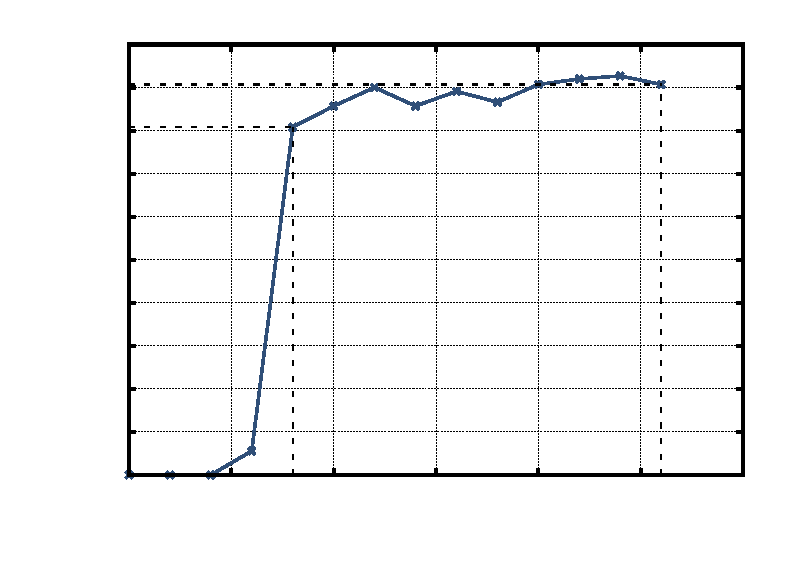
\includegraphics{plateau}}%
    \gplfronttext
  \end{picture}%
\endgroup
}	
	
	\caption{Wykres zależności liczby zliczeń od napięcia.}
	\label{wykres_plateau}
\end{figure}

Na wykres [\ref{wykres_plateau}] naniesiono punkty $(U_A,J_A)$ oraz $(U_B,J_B)$.

\begin{table}[h!]
\centering
	\begin{tabular}{|C{2cm}|C{2.5cm}|}\hline
	$J_A = 808$ & $U_A  = 1280$ V \\ \hline
	$J_B = 907$ & $U_B  = 1460$ V \\ \hline
	\end{tabular}
\end{table}


Korzystając ze wzoru \ref{nachylenie} obliczono nachylenie $\alpha = 12,25 \%$ przypadające na $180$ V. Łatwo wyliczyć, że nachylenie na 100 V wynosi:
\begin{equation*}
	\alpha = 6,73 \%
\end{equation*}
\item \textbf{Pomiar liczby zliczeń ze źródłem na zewnątrz domku pomiarowego}\\
Następnie wykonano sto pomiarów dla źródła umieszczonego w takiej odległości poza domkiem aby średnio obserwować jedno zliczenie na sekundę. Wyniki pomiarów przedstawiono na wykresie \ref{hist1}. Razem z otrzymanym rozkładem przedstawiono rozkład teoretyczny(Poissona) wynikający ze wzoru \ref{poisson}. Obliczenia oparto na wyliczonej średniej arytmetycznej $\lambda = 0,86$ zliczeń na sekundę.
\begin{figure}[h!]
	\fontsize{6}{8}\selectfont % zmniejszam czcionke
	\centering
	\resizebox{0.9\textwidth}{!}{% GNUPLOT: LaTeX picture with Postscript
\begingroup
  \makeatletter
  \providecommand\color[2][]{%
    \GenericError{(gnuplot) \space\space\space\@spaces}{%
      Package color not loaded in conjunction with
      terminal option `colourtext'%
    }{See the gnuplot documentation for explanation.%
    }{Either use 'blacktext' in gnuplot or load the package
      color.sty in LaTeX.}%
    \renewcommand\color[2][]{}%
  }%
  \providecommand\includegraphics[2][]{%
    \GenericError{(gnuplot) \space\space\space\@spaces}{%
      Package graphicx or graphics not loaded%
    }{See the gnuplot documentation for explanation.%
    }{The gnuplot epslatex terminal needs graphicx.sty or graphics.sty.}%
    \renewcommand\includegraphics[2][]{}%
  }%
  \providecommand\rotatebox[2]{#2}%
  \@ifundefined{ifGPcolor}{%
    \newif\ifGPcolor
    \GPcolortrue
  }{}%
  \@ifundefined{ifGPblacktext}{%
    \newif\ifGPblacktext
    \GPblacktextfalse
  }{}%
  % define a \g@addto@macro without @ in the name:
  \let\gplgaddtomacro\g@addto@macro
  % define empty templates for all commands taking text:
  \gdef\gplbacktext{}%
  \gdef\gplfronttext{}%
  \makeatother
  \ifGPblacktext
    % no textcolor at all
    \def\colorrgb#1{}%
    \def\colorgray#1{}%
  \else
    % gray or color?
    \ifGPcolor
      \def\colorrgb#1{\color[rgb]{#1}}%
      \def\colorgray#1{\color[gray]{#1}}%
      \expandafter\def\csname LTw\endcsname{\color{white}}%
      \expandafter\def\csname LTb\endcsname{\color{black}}%
      \expandafter\def\csname LTa\endcsname{\color{black}}%
      \expandafter\def\csname LT0\endcsname{\color[rgb]{1,0,0}}%
      \expandafter\def\csname LT1\endcsname{\color[rgb]{0,1,0}}%
      \expandafter\def\csname LT2\endcsname{\color[rgb]{0,0,1}}%
      \expandafter\def\csname LT3\endcsname{\color[rgb]{1,0,1}}%
      \expandafter\def\csname LT4\endcsname{\color[rgb]{0,1,1}}%
      \expandafter\def\csname LT5\endcsname{\color[rgb]{1,1,0}}%
      \expandafter\def\csname LT6\endcsname{\color[rgb]{0,0,0}}%
      \expandafter\def\csname LT7\endcsname{\color[rgb]{1,0.3,0}}%
      \expandafter\def\csname LT8\endcsname{\color[rgb]{0.5,0.5,0.5}}%
    \else
      % gray
      \def\colorrgb#1{\color{black}}%
      \def\colorgray#1{\color[gray]{#1}}%
      \expandafter\def\csname LTw\endcsname{\color{white}}%
      \expandafter\def\csname LTb\endcsname{\color{black}}%
      \expandafter\def\csname LTa\endcsname{\color{black}}%
      \expandafter\def\csname LT0\endcsname{\color{black}}%
      \expandafter\def\csname LT1\endcsname{\color{black}}%
      \expandafter\def\csname LT2\endcsname{\color{black}}%
      \expandafter\def\csname LT3\endcsname{\color{black}}%
      \expandafter\def\csname LT4\endcsname{\color{black}}%
      \expandafter\def\csname LT5\endcsname{\color{black}}%
      \expandafter\def\csname LT6\endcsname{\color{black}}%
      \expandafter\def\csname LT7\endcsname{\color{black}}%
      \expandafter\def\csname LT8\endcsname{\color{black}}%
    \fi
  \fi
  \setlength{\unitlength}{0.0500bp}%
  \begin{picture}(7370.00,5102.00)%
    \gplgaddtomacro\gplbacktext{%
      \csname LTb\endcsname%
      \put(814,704){\makebox(0,0)[r]{\strut{} 0}}%
      \csname LTb\endcsname%
      \put(814,1163){\makebox(0,0)[r]{\strut{} 5}}%
      \csname LTb\endcsname%
      \put(814,1622){\makebox(0,0)[r]{\strut{} 10}}%
      \csname LTb\endcsname%
      \put(814,2082){\makebox(0,0)[r]{\strut{} 15}}%
      \csname LTb\endcsname%
      \put(814,2541){\makebox(0,0)[r]{\strut{} 20}}%
      \csname LTb\endcsname%
      \put(814,3000){\makebox(0,0)[r]{\strut{} 25}}%
      \csname LTb\endcsname%
      \put(814,3459){\makebox(0,0)[r]{\strut{} 30}}%
      \csname LTb\endcsname%
      \put(814,3919){\makebox(0,0)[r]{\strut{} 35}}%
      \csname LTb\endcsname%
      \put(814,4378){\makebox(0,0)[r]{\strut{} 40}}%
      \csname LTb\endcsname%
      \put(814,4837){\makebox(0,0)[r]{\strut{} 45}}%
      \csname LTb\endcsname%
      \put(946,484){\makebox(0,0){\strut{}-1}}%
      \csname LTb\endcsname%
      \put(1807,484){\makebox(0,0){\strut{} 0}}%
      \csname LTb\endcsname%
      \put(2668,484){\makebox(0,0){\strut{} 1}}%
      \csname LTb\endcsname%
      \put(3529,484){\makebox(0,0){\strut{} 2}}%
      \csname LTb\endcsname%
      \put(4390,484){\makebox(0,0){\strut{} 3}}%
      \csname LTb\endcsname%
      \put(5251,484){\makebox(0,0){\strut{} 4}}%
      \csname LTb\endcsname%
      \put(6112,484){\makebox(0,0){\strut{} 5}}%
      \csname LTb\endcsname%
      \put(6973,484){\makebox(0,0){\strut{} 6}}%
      \put(176,2770){\rotatebox{-270}{\makebox(0,0){\strut{}Częstość}}}%
      \put(3959,154){\makebox(0,0){\strut{}Liczba zliczeń na sekundę}}%
    }%
    \gplgaddtomacro\gplfronttext{%
      \csname LTb\endcsname%
      \put(5986,4664){\makebox(0,0)[r]{\strut{}Otrzymany rozkład}}%
      \csname LTb\endcsname%
      \put(1678,4424){\makebox(0,0){\strut{}40}}%
      \put(2539,4607){\makebox(0,0){\strut{}42}}%
      \put(3400,1760){\makebox(0,0){\strut{}11}}%
      \put(4261,1301){\makebox(0,0){\strut{}6}}%
      \put(5122,842){\makebox(0,0){\strut{}1}}%
      \put(5983,750){\makebox(0,0){\strut{}0}}%
      \csname LTb\endcsname%
      \put(5986,4444){\makebox(0,0)[r]{\strut{}Rozkład teoretyczny}}%
      \csname LTb\endcsname%
      \put(1936,4637){\makebox(0,0){\strut{}42.32}}%
      \put(2797,4092){\makebox(0,0){\strut{}36.39}}%
      \put(3658,2186){\makebox(0,0){\strut{}15.64}}%
      \put(4519,1161){\makebox(0,0){\strut{}4.48}}%
      \put(5380,838){\makebox(0,0){\strut{}0.96}}%
      \put(6241,765){\makebox(0,0){\strut{}0.16}}%
    }%
    \gplbacktext
    \put(0,0){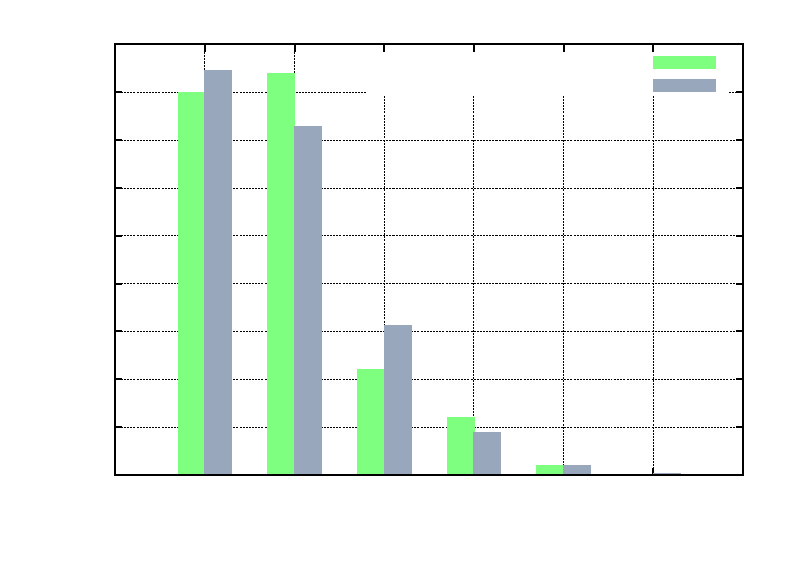
\includegraphics{histogram1}}%
    \gplfronttext
  \end{picture}%
\endgroup
}	
	
	\caption{Histogram}
	\label{hist1}
\end{figure}

Obliczono wartość $\chi^2$ korzystając ze wzoru \ref{chi}. Otrzymano wynik $3,04$ następnie korzystając z tablic statystycznych [\ref{przybycien}] odczytano wartość krytyczną dla przedziału ufności $0,05$ oraz liczby stopni swobody $5$ wynikającej z liczby obserwacji $6$ pomniejszonej o jeden estymowany parametr. Odczytana wartość $\chi^2_\alpha = 4.35 $ jest mniejsza od $\chi^2$ zatem nie ma podstaw by odrzucić hipotezę iż dany rozkład jest rozkładem Poissona.

\item \textbf{Pomiar liczby zliczeń ze źródłem na najniższym poziomie domku pomiarowego}
Badana źródło umieszczono wewnątrz domku pomiarowego tak, aby obserwować około 5 zliczeń w przedziale czasowym trwającym $1$ sekundę. Wykonano 100 takich pomiarów. Na rysunku \ref{hist2} przedstawiono histogram otrzymanego rozkładu oraz histogram rozkładu teoretycznego o $\lambda = 4,75$. W tabeli \ref{czestosc2} przedstawiono wyniki obliczeń składowych $\chi^2$ oraz ostateczny wynik.


\begin{figure}[h!]
	\fontsize{6}{8}\selectfont % zmniejszam czcionke
	\centering
	\resizebox{0.8\textwidth}{!}{% GNUPLOT: LaTeX picture with Postscript
\begingroup
  \makeatletter
  \providecommand\color[2][]{%
    \GenericError{(gnuplot) \space\space\space\@spaces}{%
      Package color not loaded in conjunction with
      terminal option `colourtext'%
    }{See the gnuplot documentation for explanation.%
    }{Either use 'blacktext' in gnuplot or load the package
      color.sty in LaTeX.}%
    \renewcommand\color[2][]{}%
  }%
  \providecommand\includegraphics[2][]{%
    \GenericError{(gnuplot) \space\space\space\@spaces}{%
      Package graphicx or graphics not loaded%
    }{See the gnuplot documentation for explanation.%
    }{The gnuplot epslatex terminal needs graphicx.sty or graphics.sty.}%
    \renewcommand\includegraphics[2][]{}%
  }%
  \providecommand\rotatebox[2]{#2}%
  \@ifundefined{ifGPcolor}{%
    \newif\ifGPcolor
    \GPcolortrue
  }{}%
  \@ifundefined{ifGPblacktext}{%
    \newif\ifGPblacktext
    \GPblacktextfalse
  }{}%
  % define a \g@addto@macro without @ in the name:
  \let\gplgaddtomacro\g@addto@macro
  % define empty templates for all commands taking text:
  \gdef\gplbacktext{}%
  \gdef\gplfronttext{}%
  \makeatother
  \ifGPblacktext
    % no textcolor at all
    \def\colorrgb#1{}%
    \def\colorgray#1{}%
  \else
    % gray or color?
    \ifGPcolor
      \def\colorrgb#1{\color[rgb]{#1}}%
      \def\colorgray#1{\color[gray]{#1}}%
      \expandafter\def\csname LTw\endcsname{\color{white}}%
      \expandafter\def\csname LTb\endcsname{\color{black}}%
      \expandafter\def\csname LTa\endcsname{\color{black}}%
      \expandafter\def\csname LT0\endcsname{\color[rgb]{1,0,0}}%
      \expandafter\def\csname LT1\endcsname{\color[rgb]{0,1,0}}%
      \expandafter\def\csname LT2\endcsname{\color[rgb]{0,0,1}}%
      \expandafter\def\csname LT3\endcsname{\color[rgb]{1,0,1}}%
      \expandafter\def\csname LT4\endcsname{\color[rgb]{0,1,1}}%
      \expandafter\def\csname LT5\endcsname{\color[rgb]{1,1,0}}%
      \expandafter\def\csname LT6\endcsname{\color[rgb]{0,0,0}}%
      \expandafter\def\csname LT7\endcsname{\color[rgb]{1,0.3,0}}%
      \expandafter\def\csname LT8\endcsname{\color[rgb]{0.5,0.5,0.5}}%
    \else
      % gray
      \def\colorrgb#1{\color{black}}%
      \def\colorgray#1{\color[gray]{#1}}%
      \expandafter\def\csname LTw\endcsname{\color{white}}%
      \expandafter\def\csname LTb\endcsname{\color{black}}%
      \expandafter\def\csname LTa\endcsname{\color{black}}%
      \expandafter\def\csname LT0\endcsname{\color{black}}%
      \expandafter\def\csname LT1\endcsname{\color{black}}%
      \expandafter\def\csname LT2\endcsname{\color{black}}%
      \expandafter\def\csname LT3\endcsname{\color{black}}%
      \expandafter\def\csname LT4\endcsname{\color{black}}%
      \expandafter\def\csname LT5\endcsname{\color{black}}%
      \expandafter\def\csname LT6\endcsname{\color{black}}%
      \expandafter\def\csname LT7\endcsname{\color{black}}%
      \expandafter\def\csname LT8\endcsname{\color{black}}%
    \fi
  \fi
  \setlength{\unitlength}{0.0500bp}%
  \begin{picture}(7370.00,5102.00)%
    \gplgaddtomacro\gplbacktext{%
      \csname LTb\endcsname%
      \put(814,704){\makebox(0,0)[r]{\strut{} 0}}%
      \csname LTb\endcsname%
      \put(814,1531){\makebox(0,0)[r]{\strut{} 5}}%
      \csname LTb\endcsname%
      \put(814,2357){\makebox(0,0)[r]{\strut{} 10}}%
      \csname LTb\endcsname%
      \put(814,3184){\makebox(0,0)[r]{\strut{} 15}}%
      \csname LTb\endcsname%
      \put(814,4010){\makebox(0,0)[r]{\strut{} 20}}%
      \csname LTb\endcsname%
      \put(814,4837){\makebox(0,0)[r]{\strut{} 25}}%
      \csname LTb\endcsname%
      \put(946,484){\makebox(0,0){\strut{}-2}}%
      \csname LTb\endcsname%
      \put(1699,484){\makebox(0,0){\strut{} 0}}%
      \csname LTb\endcsname%
      \put(2453,484){\makebox(0,0){\strut{} 2}}%
      \csname LTb\endcsname%
      \put(3206,484){\makebox(0,0){\strut{} 4}}%
      \csname LTb\endcsname%
      \put(3960,484){\makebox(0,0){\strut{} 6}}%
      \csname LTb\endcsname%
      \put(4713,484){\makebox(0,0){\strut{} 8}}%
      \csname LTb\endcsname%
      \put(5466,484){\makebox(0,0){\strut{} 10}}%
      \csname LTb\endcsname%
      \put(6220,484){\makebox(0,0){\strut{} 12}}%
      \csname LTb\endcsname%
      \put(6973,484){\makebox(0,0){\strut{} 14}}%
      \put(176,2770){\rotatebox{-270}{\makebox(0,0){\strut{}Częstość}}}%
      \put(3959,154){\makebox(0,0){\strut{}Liczba zliczeń na sekundę}}%
    }%
    \gplgaddtomacro\gplfronttext{%
      \csname LTb\endcsname%
      \put(5986,4664){\makebox(0,0)[r]{\strut{}Otrzymany rozkład}}%
      \csname LTb\endcsname%
      \put(5986,4444){\makebox(0,0)[r]{\strut{}Rozkład teoretyczny}}%
    }%
    \gplbacktext
    \put(0,0){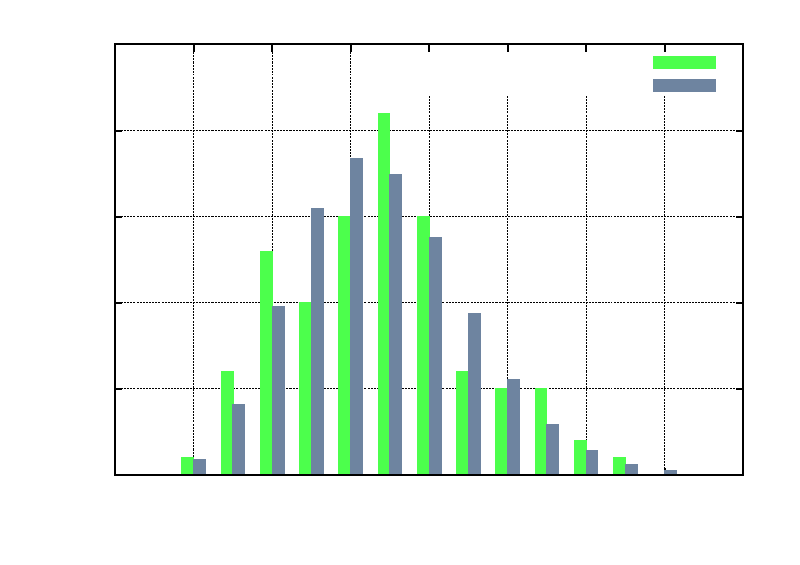
\includegraphics{histogram2}}%
    \gplfronttext
  \end{picture}%
\endgroup
}
	
	\caption{Histogramy otrzymanego rozkładu oraz rozkładu Poissona o $\lambda = 4,75$}
	\label{hist2}
\end{figure}


\begin{table}[h!]
\centering
\label{czestosc2}
\caption{Wyniki pomiarów liczby zliczeń dla źródła na najniższym poziomie domku pomiarowego}
	\begin{tabular}{|C{2cm}|C{2cm}|C{2cm}|C{3cm}|}\hline
			Liczba zliczeń & Częstość & Częstość teoretyczna & $(x-x_{oi})^2/x_{oi}$ \\ \hline
			0	&	1		&	0,87	&	0,02 \\ \hline
			1	&	6		&	4,11	&	0,87 \\ \hline
			2	&	13		&	9,76	&	1,08 \\ \hline
			3	&	10		&	15,45	&	1,92 \\ \hline
			4	&	15		&	18,35	&	0,61 \\ \hline
			5	&	21		&	17,43	&	0,73 \\ \hline
			6	&	15		&	13,80	&	0,10 \\ \hline
			7	&	6		&	9,37	&	1,21 \\ \hline
			8	&	5		&	5,56	&	0,06 \\ \hline
			9	&	5		&	2,93	&	1,45 \\ \hline
			10	&	2		&	1,39	&	0,26 \\ \hline
			11	&	1		&	0,60	&	0,26 \\ \hline
			12	&	0		&	0,24	&	0,24 \\ \hline
				&			&	$\boldsymbol{\chi^2}$		& \textbf{8,82} \\ \hline

	\end{tabular}

\end{table}
Tablice statystyczne \ref{przybycien} przewidują dla 12 stopni swobody i przedziału ufności 0,05 wartość krytyczną: $21,03$, która jest mniejsza od wyliczonej $\chi^2$. Nie mamy zatem podstaw aby odrzucić hipotezę, że ten rozkład jest rozkładem Poissona.
\newpage
\item \textbf{Źródło umieszczone bardzo blisko licznika} \\
	Źródło umieszczono na najwyższym szczeblu domku pomiarowego. Wykonano 200 pomiarów o czasie trwania równym 1s.
Otrzymane wyniki przedstawiono tabeli \ref{wyniki_gauss}. Otrzymane rozkłady przedstawiono na wykresie \ref{hist3}. Przy pomocy arkusza kalkulacyjnego wyliczono wartość oczekiwaną $\mu = 543,40$ oraz odchylenie standardowe $\sigma = 18,30$. Dla liczby stopni swobody równej 23 oraz przedziału ufności tablice statystyczne przewidują wartość $\chi^2_\alpha = 35,17$. Jak wynika z tabeli \ref{wyniki_gauss} otrzymana wartość $\chi^2 = 23,22$ jest mniejsza od wartości krytycznej, zatem tak jak w poprzednich przypadkach nie mamy podstaw odrzucić hipotezy, że otrzymany rozkład jest rozkładem normalnym.

\begin{table}[h!]
\centering
\label{wyniki_gauss}
\caption{Wyniki pomiarów liczby zliczeń dla źródła umieszczonego bardzo blisko licznika.}
	\begin{tabular}{|C{2cm}|C{2cm}|C{2cm}|C{3cm}|C{3cm}|}\hline
			&	Przedział	&	Częstość		& Wartość teoretyczna  & $(x-x_{oi})^2/x_{oi}$ \\ \hline
		1	&	$(-\infty)–500$&	0	&	1,31	&	1,31 \\ \hline
		2	&	500-505 &	1	&	2,41	&	0,83 \\ \hline
		3	&	505-510 &	2	&	4,12	&	1,09 \\ \hline
		4	&	510-515 &	7	&	6,54	&	0,03 \\ \hline
		5	&	515-520 &	6	&	9,63	&	1,37 \\ \hline
		6	&	520-525 &	13	&	13,15	&	0,00 \\ \hline
		7	&	525-530 &	23	&	16,68	&	2,40 \\ \hline
		8	&	530-535 &	20	&	19,63	&	0,01 \\ \hline
		9	&	535-540 &	29	&	21,43	&	2,67 \\ \hline
		10	&	540-545 &	21	&	21,72	&	0,02 \\ \hline
		11	&	545-550 &	14	&	20,43	&	2,02 \\ \hline
		12	&	550-555 &	11	&	17,83	&	2,62 \\ \hline
		13	&	555-560 &	15	&	14,44	&	0,02 \\ \hline
		14	&	560-565 &	12	&	10,86	&	0,12 \\ \hline
		15	&	565-570 &	12	&	7,58	&	2,58 \\ \hline
		16	&	570-575 &	7	&	4,90	&	0,90 \\ \hline
		17	&	575-580 &	2	&	2,95	&	0,30 \\ \hline
		18	&	580-585 &	1	&	1,64	&	0,25 \\ \hline
		19	&	585-590 &	1	&	0,85	&	0,03 \\ \hline
		20	&	590-595 &	1	&	0,41	&	0,86 \\ \hline
		21	&	595-600 &	1	&	0,18	&	3,68 \\ \hline
		22	&	600-605 &	0	&	0,08	&	0,08 \\ \hline
		23	&	605-610 &	0	&	0,03	&	0,03 \\ \hline
		24	&	$ 610-(+\infty)$&	0	&	0,01	&	0,01 \\ \hline
			&		&		&	$\boldsymbol{\chi^2}$		& \textbf{23,22} \\ \hline


	\end{tabular}

\end{table}


\begin{figure}[h!]
	\fontsize{6}{8}\selectfont % zmniejszam czcionke
	\centering
	\resizebox{0.9\textwidth}{!}{% GNUPLOT: LaTeX picture with Postscript
\begingroup
  \makeatletter
  \providecommand\color[2][]{%
    \GenericError{(gnuplot) \space\space\space\@spaces}{%
      Package color not loaded in conjunction with
      terminal option `colourtext'%
    }{See the gnuplot documentation for explanation.%
    }{Either use 'blacktext' in gnuplot or load the package
      color.sty in LaTeX.}%
    \renewcommand\color[2][]{}%
  }%
  \providecommand\includegraphics[2][]{%
    \GenericError{(gnuplot) \space\space\space\@spaces}{%
      Package graphicx or graphics not loaded%
    }{See the gnuplot documentation for explanation.%
    }{The gnuplot epslatex terminal needs graphicx.sty or graphics.sty.}%
    \renewcommand\includegraphics[2][]{}%
  }%
  \providecommand\rotatebox[2]{#2}%
  \@ifundefined{ifGPcolor}{%
    \newif\ifGPcolor
    \GPcolortrue
  }{}%
  \@ifundefined{ifGPblacktext}{%
    \newif\ifGPblacktext
    \GPblacktextfalse
  }{}%
  % define a \g@addto@macro without @ in the name:
  \let\gplgaddtomacro\g@addto@macro
  % define empty templates for all commands taking text:
  \gdef\gplbacktext{}%
  \gdef\gplfronttext{}%
  \makeatother
  \ifGPblacktext
    % no textcolor at all
    \def\colorrgb#1{}%
    \def\colorgray#1{}%
  \else
    % gray or color?
    \ifGPcolor
      \def\colorrgb#1{\color[rgb]{#1}}%
      \def\colorgray#1{\color[gray]{#1}}%
      \expandafter\def\csname LTw\endcsname{\color{white}}%
      \expandafter\def\csname LTb\endcsname{\color{black}}%
      \expandafter\def\csname LTa\endcsname{\color{black}}%
      \expandafter\def\csname LT0\endcsname{\color[rgb]{1,0,0}}%
      \expandafter\def\csname LT1\endcsname{\color[rgb]{0,1,0}}%
      \expandafter\def\csname LT2\endcsname{\color[rgb]{0,0,1}}%
      \expandafter\def\csname LT3\endcsname{\color[rgb]{1,0,1}}%
      \expandafter\def\csname LT4\endcsname{\color[rgb]{0,1,1}}%
      \expandafter\def\csname LT5\endcsname{\color[rgb]{1,1,0}}%
      \expandafter\def\csname LT6\endcsname{\color[rgb]{0,0,0}}%
      \expandafter\def\csname LT7\endcsname{\color[rgb]{1,0.3,0}}%
      \expandafter\def\csname LT8\endcsname{\color[rgb]{0.5,0.5,0.5}}%
    \else
      % gray
      \def\colorrgb#1{\color{black}}%
      \def\colorgray#1{\color[gray]{#1}}%
      \expandafter\def\csname LTw\endcsname{\color{white}}%
      \expandafter\def\csname LTb\endcsname{\color{black}}%
      \expandafter\def\csname LTa\endcsname{\color{black}}%
      \expandafter\def\csname LT0\endcsname{\color{black}}%
      \expandafter\def\csname LT1\endcsname{\color{black}}%
      \expandafter\def\csname LT2\endcsname{\color{black}}%
      \expandafter\def\csname LT3\endcsname{\color{black}}%
      \expandafter\def\csname LT4\endcsname{\color{black}}%
      \expandafter\def\csname LT5\endcsname{\color{black}}%
      \expandafter\def\csname LT6\endcsname{\color{black}}%
      \expandafter\def\csname LT7\endcsname{\color{black}}%
      \expandafter\def\csname LT8\endcsname{\color{black}}%
    \fi
  \fi
  \setlength{\unitlength}{0.0500bp}%
  \begin{picture}(9070.00,5102.00)%
    \gplgaddtomacro\gplbacktext{%
      \csname LTb\endcsname%
      \put(814,704){\makebox(0,0)[r]{\strut{} 0}}%
      \csname LTb\endcsname%
      \put(814,1393){\makebox(0,0)[r]{\strut{} 5}}%
      \csname LTb\endcsname%
      \put(814,2082){\makebox(0,0)[r]{\strut{} 10}}%
      \csname LTb\endcsname%
      \put(814,2771){\makebox(0,0)[r]{\strut{} 15}}%
      \csname LTb\endcsname%
      \put(814,3459){\makebox(0,0)[r]{\strut{} 20}}%
      \csname LTb\endcsname%
      \put(814,4148){\makebox(0,0)[r]{\strut{} 25}}%
      \csname LTb\endcsname%
      \put(814,4837){\makebox(0,0)[r]{\strut{} 30}}%
      \csname LTb\endcsname%
      \put(946,484){\makebox(0,0){\strut{} 500}}%
      \csname LTb\endcsname%
      \put(2050,484){\makebox(0,0){\strut{} 520}}%
      \csname LTb\endcsname%
      \put(3154,484){\makebox(0,0){\strut{} 540}}%
      \csname LTb\endcsname%
      \put(4258,484){\makebox(0,0){\strut{} 560}}%
      \csname LTb\endcsname%
      \put(5361,484){\makebox(0,0){\strut{} 580}}%
      \csname LTb\endcsname%
      \put(6465,484){\makebox(0,0){\strut{} 600}}%
      \csname LTb\endcsname%
      \put(7569,484){\makebox(0,0){\strut{} 620}}%
      \csname LTb\endcsname%
      \put(8673,484){\makebox(0,0){\strut{} 640}}%
      \put(176,2770){\rotatebox{-270}{\makebox(0,0){\strut{}Częstość}}}%
      \put(4809,154){\makebox(0,0){\strut{}Liczba zliczeń na sekundę}}%
    }%
    \gplgaddtomacro\gplfronttext{%
      \csname LTb\endcsname%
      \put(7686,4664){\makebox(0,0)[r]{\strut{}Otrzymany rozkład}}%
      \csname LTb\endcsname%
      \put(7686,4444){\makebox(0,0)[r]{\strut{}Rozkład teoretyczny}}%
    }%
    \gplbacktext
    \put(0,0){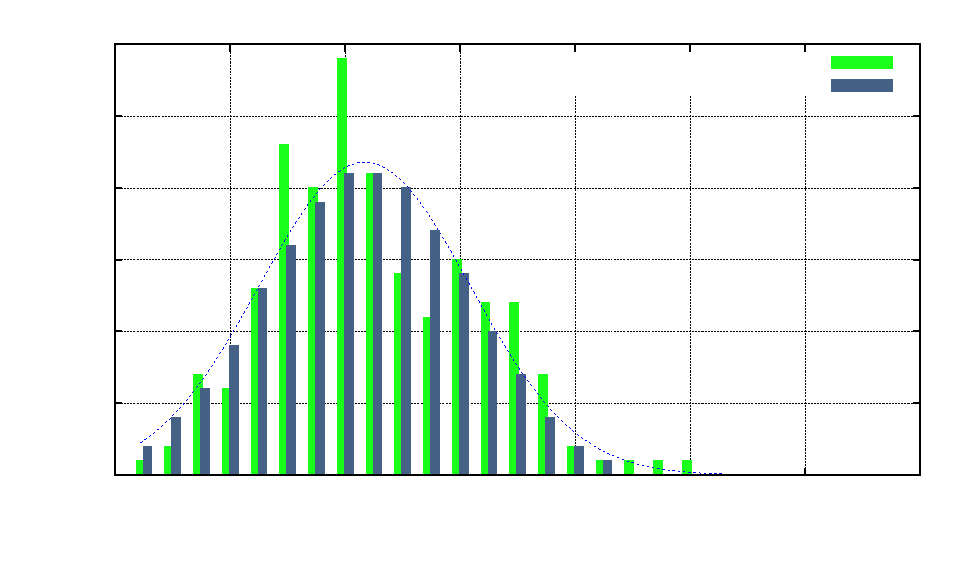
\includegraphics{histogram3}}%
    \gplfronttext
  \end{picture}%
\endgroup
}
	
	\caption{Histogramy otrzymanego rozkładu oraz rozkładu Gaussa}
	\label{hist3}
\end{figure}




\end{itemize}
\newpage
%%%%%%%%%%%%%%%%%%%%%%%%%%%% SREBRO %%%%%%%%%%%%%%%%%%%%%%%%%%%%%%%%%

\section{Czas połowicznego rozpadu srebra.}
\subsection{Cel ćwiczenia.}
   Celem ćwiczenia jest doświadczalne wyznaczenie czasu połowicznego rozpadu płytki srebra zaaktywowanej wcześniej przy pomocy neutronów.

\subsection{Wstęp.}
Doświadczalne wyznaczenie czasu połowicznego rozpadu poprzez narysowanie krzywej rozpadu jest możliwe dla izotopów o krótkim czasie życia (czas połowicznego rozpadu rzędu kilkudziesięciu sekund lub kilku minut).
Przykładami takich izotopów mogą być aktywowane izotopy srebra.

W przyrodzie srebro występuje w postaci dwóch stabilnych izotopów: $^{107}$Ag (51.35\%) oraz $^{109}$Ag (48.65\%). Pod wpływem bombardowania neutronami (termicznymi lub szybkimi) srebro ulega aktywacji poprzez pochłonięcie neutronu:\\
\[^{107}\text{Ag} + \text{n} \to ^{108}\text{Ag} + \gamma
\]
\[^{109}\text{Ag} + \text{n} \to ^{110}\text{Ag} + \gamma
\]\\\\
Oprócz powyższych izotopów powstają jeszcze $^{108m}$Ag oraz $^{110m}$Ag jednak ich czasy połowicznego rozpadu to odpowiednio 418 lat oraz 250 dni, więc nie wpływają one na wyniki naszego doświadczenia.\\
Powstałe w wyniku aktywacji izotopy mają czas połowicznego rozpadu (tablicowy \cite{1}) równy 2.37 min dla $^{108}$Ag oraz 24.6 s dla $^{110}$Ag, co w dalszej części doświadczenia wyznaczano. Oba izotopy ulegają rozpadowi $\beta ^-$. \\\\
Powyższe rozpady opisuje prawo rozpadu promioniotwórczego:
\begin{equation}
N(t) = N_0 \exp^{-\lambda t}
\end{equation}
Po przekształceniu możemy je zapisać w postaci:
\begin{equation}
\ln N = -\lambda t + \ln N_0
\label{wz_rozpad_log}
\end{equation}
Z powyższego równania wynika, że dla rozpadu pojedynczego izotopu narysowany w skali półlogarytmicznej wykres liczby rozpadów od czasu powinien być linią prostą. Wyznaczając współczynnik kierunkowy tej prostej oraz korzystając z definicji czasu połowicznego rozpadu możemy go wyznaczyć jako:
\begin{equation}
\tau = \frac{\ln 2}{\lambda}
\label{wz_tau}
\end{equation}
Gdzie:\\
$\tau$ - czas połowicznego rozpadu\\
$\lambda $ - stała rozpadu wyznaczona jako współczynnik nachylenia prostej\\

W przypadku, gdy w badanej próbce znajduję się kilka izotopów wykorzystujemy różnicę w czasach połowicznego rozpadu ( po czasie około 3.5$\tau _1$ pierwszy z izotopów całkowicie się rozpadnie przy czym ciągle będziemy rejestrować rozpady drugiego izotopu). Narysowany w skali półlogarytmicznej wykres powinien wyglądać mniej więcej tak jak ten na Rysunku \ref{schemat}. \\
Krzywa 1 na rysunku reprezentuję wyznaczoną krzywą, celem znalezienia prostej $2$ należy wyznaczyć (np. metodą najmniejszych kwadratów) równanie prostej $1'$, a następnie ekstrapolować ją punktu $t=0$. Jeżeli przez $t_1$ oznaczymy czas, w którym izotop o krótszym czasie życia uległ całkowitemu rozpadowi, to prostą $1'$ będziemy dopasowywać do punktów zaczynających się od tego właśnie punktu. Kolejnym krokiem jest odjęcie prostej $1'$ od danych pomiarowych i do otrzymanych punktów z przedziału od $t=0$ do $t_1$ ponownie dopasowujemy prostą.\\
Otrzymane proste to proste rozpadu poszczególnych izotopów w skali półlogarytmicznej, czasy ich połowicznego rozpadu wyznaczamy ze wzoru (\ref{wz_tau})

\begin{figure}[h]
	\centering
	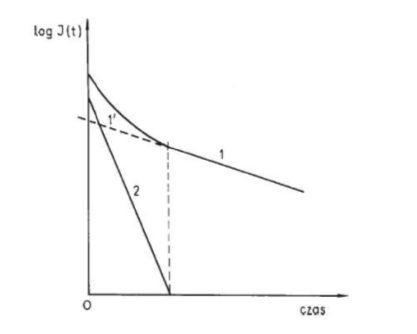
\includegraphics[width=0.7\textwidth]{images/schemat.png}
	\caption{Schemat wykresu półlogarytmicznego dla rozpadu dwóch izotopów różniących się czasami połowicznego rozpadu.}
	\label{schemat}
\end{figure}



\subsection{Wykonanie ćwiczenia.}
Doświadczenie rozpoczęto od włożenia srebrnej płytki do źródła neutronów na czas 10 minut.\\
Następnie po upływie tego czasu bardzo szybko (około 20s upłynęło od wyjęcia płytki do rozpoczęcia pomiarów) wyjęto płytkę i umieszczono w detektorze  rozpoczynając pomiary. Liczbę zliczeń notowano w odstępie 6 sekund, wyniki przedstawia tabela \ref{wyniki_dat} oraz wykres przedstawiony na Rysunku \ref{wykres_zliczenia_czas}. Czas $t_1$ całkowitego rozpadu srebra $^{110}$Ag oszacowano na 150s.\\
Do dalszych obliczeń przyjęto, że wielkości związane z $^{108}$Ag będą miały indeks 1 natomiast związane z $^{110}$Ag indeks 2.\\

\begin{figure}[h!]
	\fontsize{6}{8}\selectfont % zmniejszam czcionke
	\centering
	\resizebox{1.0\textwidth}{!}{% GNUPLOT: LaTeX picture with Postscript
\begingroup
  \makeatletter
  \providecommand\color[2][]{%
    \GenericError{(gnuplot) \space\space\space\@spaces}{%
      Package color not loaded in conjunction with
      terminal option `colourtext'%
    }{See the gnuplot documentation for explanation.%
    }{Either use 'blacktext' in gnuplot or load the package
      color.sty in LaTeX.}%
    \renewcommand\color[2][]{}%
  }%
  \providecommand\includegraphics[2][]{%
    \GenericError{(gnuplot) \space\space\space\@spaces}{%
      Package graphicx or graphics not loaded%
    }{See the gnuplot documentation for explanation.%
    }{The gnuplot epslatex terminal needs graphicx.sty or graphics.sty.}%
    \renewcommand\includegraphics[2][]{}%
  }%
  \providecommand\rotatebox[2]{#2}%
  \@ifundefined{ifGPcolor}{%
    \newif\ifGPcolor
    \GPcolortrue
  }{}%
  \@ifundefined{ifGPblacktext}{%
    \newif\ifGPblacktext
    \GPblacktextfalse
  }{}%
  % define a \g@addto@macro without @ in the name:
  \let\gplgaddtomacro\g@addto@macro
  % define empty templates for all commands taking text:
  \gdef\gplbacktext{}%
  \gdef\gplfronttext{}%
  \makeatother
  \ifGPblacktext
    % no textcolor at all
    \def\colorrgb#1{}%
    \def\colorgray#1{}%
  \else
    % gray or color?
    \ifGPcolor
      \def\colorrgb#1{\color[rgb]{#1}}%
      \def\colorgray#1{\color[gray]{#1}}%
      \expandafter\def\csname LTw\endcsname{\color{white}}%
      \expandafter\def\csname LTb\endcsname{\color{black}}%
      \expandafter\def\csname LTa\endcsname{\color{black}}%
      \expandafter\def\csname LT0\endcsname{\color[rgb]{1,0,0}}%
      \expandafter\def\csname LT1\endcsname{\color[rgb]{0,1,0}}%
      \expandafter\def\csname LT2\endcsname{\color[rgb]{0,0,1}}%
      \expandafter\def\csname LT3\endcsname{\color[rgb]{1,0,1}}%
      \expandafter\def\csname LT4\endcsname{\color[rgb]{0,1,1}}%
      \expandafter\def\csname LT5\endcsname{\color[rgb]{1,1,0}}%
      \expandafter\def\csname LT6\endcsname{\color[rgb]{0,0,0}}%
      \expandafter\def\csname LT7\endcsname{\color[rgb]{1,0.3,0}}%
      \expandafter\def\csname LT8\endcsname{\color[rgb]{0.5,0.5,0.5}}%
    \else
      % gray
      \def\colorrgb#1{\color{black}}%
      \def\colorgray#1{\color[gray]{#1}}%
      \expandafter\def\csname LTw\endcsname{\color{white}}%
      \expandafter\def\csname LTb\endcsname{\color{black}}%
      \expandafter\def\csname LTa\endcsname{\color{black}}%
      \expandafter\def\csname LT0\endcsname{\color{black}}%
      \expandafter\def\csname LT1\endcsname{\color{black}}%
      \expandafter\def\csname LT2\endcsname{\color{black}}%
      \expandafter\def\csname LT3\endcsname{\color{black}}%
      \expandafter\def\csname LT4\endcsname{\color{black}}%
      \expandafter\def\csname LT5\endcsname{\color{black}}%
      \expandafter\def\csname LT6\endcsname{\color{black}}%
      \expandafter\def\csname LT7\endcsname{\color{black}}%
      \expandafter\def\csname LT8\endcsname{\color{black}}%
    \fi
  \fi
  \setlength{\unitlength}{0.0500bp}%
  \begin{picture}(7370.00,5102.00)%
    \gplgaddtomacro\gplbacktext{%
      \csname LTb\endcsname%
      \put(550,704){\makebox(0,0)[r]{\strut{}$1$}}%
      \csname LTb\endcsname%
      \put(550,1294){\makebox(0,0)[r]{\strut{}$2$}}%
      \csname LTb\endcsname%
      \put(550,1885){\makebox(0,0)[r]{\strut{}$3$}}%
      \csname LTb\endcsname%
      \put(550,2475){\makebox(0,0)[r]{\strut{}$4$}}%
      \csname LTb\endcsname%
      \put(550,3066){\makebox(0,0)[r]{\strut{}$5$}}%
      \csname LTb\endcsname%
      \put(550,3656){\makebox(0,0)[r]{\strut{}$6$}}%
      \csname LTb\endcsname%
      \put(550,4247){\makebox(0,0)[r]{\strut{}$7$}}%
      \csname LTb\endcsname%
      \put(550,4837){\makebox(0,0)[r]{\strut{}$8$}}%
      \csname LTb\endcsname%
      \put(682,484){\makebox(0,0){\strut{}$0$}}%
      \csname LTb\endcsname%
      \put(1468,484){\makebox(0,0){\strut{}$100$}}%
      \csname LTb\endcsname%
      \put(2255,484){\makebox(0,0){\strut{}$200$}}%
      \csname LTb\endcsname%
      \put(3041,484){\makebox(0,0){\strut{}$300$}}%
      \csname LTb\endcsname%
      \put(3828,484){\makebox(0,0){\strut{}$400$}}%
      \csname LTb\endcsname%
      \put(4614,484){\makebox(0,0){\strut{}$500$}}%
      \csname LTb\endcsname%
      \put(5400,484){\makebox(0,0){\strut{}$600$}}%
      \csname LTb\endcsname%
      \put(6187,484){\makebox(0,0){\strut{}$700$}}%
      \csname LTb\endcsname%
      \put(6973,484){\makebox(0,0){\strut{}$800$}}%
      \put(176,2770){\rotatebox{-270}{\makebox(0,0){\strut{}log(N)}}}%
      \put(3827,154){\makebox(0,0){\strut{}Czas [s]}}%
    }%
    \gplgaddtomacro\gplfronttext{%
      \csname LTb\endcsname%
      \put(5986,4664){\makebox(0,0)[r]{\strut{}$^{108}$Ag}}%
      \csname LTb\endcsname%
      \put(5986,4444){\makebox(0,0)[r]{\strut{}$^{110}$Ag}}%
    }%
    \gplbacktext
    \put(0,0){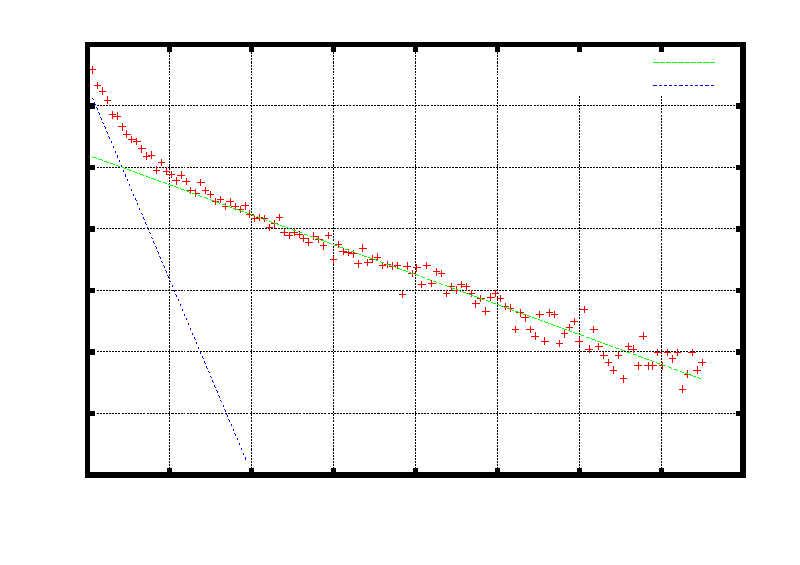
\includegraphics{srebro}}%
    \gplfronttext
  \end{picture}%
\endgroup
}	
	
	\caption{Częstość zliczeń w skali logarytmicznej z naniesionymi prostymi odpowiadającymi rozpadom poszczególnych izotopów srebra.}
	\label{wykres_zliczenia_czas}
\end{figure}

Do danych pomiarowych dla czasu $t$ większego od 150 sekund dopasowano prostą odpowiadającą rozpadowi $^{108}$Ag : \\
\[a_1 = -4.864 \pm 0.085 \cdot 10^{-3}
\]
\[	b_1 = 6.205 \pm 0.041
\]
Porównując współczynnik $a_1$ ze wzorem (\ref{wz_rozpad_log}) otrzymujemy:\\
$\lambda _1 =  4.864 \pm 0.085 \cdot 10^{-3}$\\\\

W kolejnym kroku odjęto od danych pomiarowych wartości funkcji $a_1 x + b_1$ i do otrzymanych punktów w zakresie [0:150] sekund dopasowano prostą odpowiadającą rozpadowi $^{110}$Ag :
\[a_2 = -0.0314 \pm 0.0017
\]
\[b_2 = 7.32 \pm 0.13
\]
Ponownie porównując prostą ze wzorem (\ref{wz_rozpad_log}) otrzymujemy:\\
$\lambda _2 = 0.0314 \pm 0.0017$

W ostatnim kroku korzystając ze wzoru (\ref{wz_tau}) oraz z prawa przenoszenia niepewności pomiarowej wyznaczono czasy połowicznego rozpadu.
\begin{equation}
u(\tau) = \sqrt{ \Big[ \frac{-\ln 2}{\lambda ^2}u(\lambda) \Big]^2 }
\label{wz_niepewnosc}
\end{equation}

\noindent
Wyliczone wartości dla $^{108}$Ag:\\
\[\tau _1 = 142.5 \pm 2.5\text{ s}
\]
\[\tau _{1tab} = 142.2 \text{s}
\]
\\\\
oraz dla $^{110}$Ag:\\
\[\tau _2 = 22.1 \pm 1.2 \text{s}
\]
\[\tau _{2tab} = 24.6 \text{s}
\]


\subsection{Wnioski.}
Wartości możemy uznać za równe jeżeli moduł z różnicy tych wartości jest mniejszy od niepewności wyznaczenia wartości pomnożonej przez stałą $k$ (przyjmujemy $k$=2). \\
$|\tau _1 -\tau _{1tab}| = 0.3$  $k\cdot u(\tau _1)=  5$ \\
$0.3 < 5$\\\\
Tak więc dla $^{108}$Ag wyniki uzyskane doświadczalnie są zgodne z wartościami tablicowymi.\\\\

\noindent
$|\tau _2 -\tau _{2tab}| = 2.5$  $k\cdot u(\tau _2)=  2.4$ \\
$2.5 \not< 2.4$\\\\
Wartości wyznaczone dla $^{110}$Ag nie są zgodne z wartościami tablicowymi dla $k$=2, jednak jak widać różnica jest niewielka. Wpływ na wynik ma również bardzo krótki czas życia $^{110}$Ag, być może gdyby szybciej umieszczono próbkę w detektorze udało by się dokładniej wyznaczyć czas połowicznego rozpadu i z większą dokładnością.  \\
Przedstawiona powyżej metoda jest dobrym sposobem na wyznaczenie czasu połowicznego rozpadu izotopów których czas życia jest niewielki. Szczególnie dokładny wynik otrzymaliśmy dla izotopu $^{108}$Ag.
















\end{document}





%http://nucleardata.nuclear.lu.se/toi/
%do bibliografii






